% REV00 Tue 04 May 2021 13:55:16 WIB
% START Tue 04 May 2021 13:55:16 WIB

\chapter{XXX}

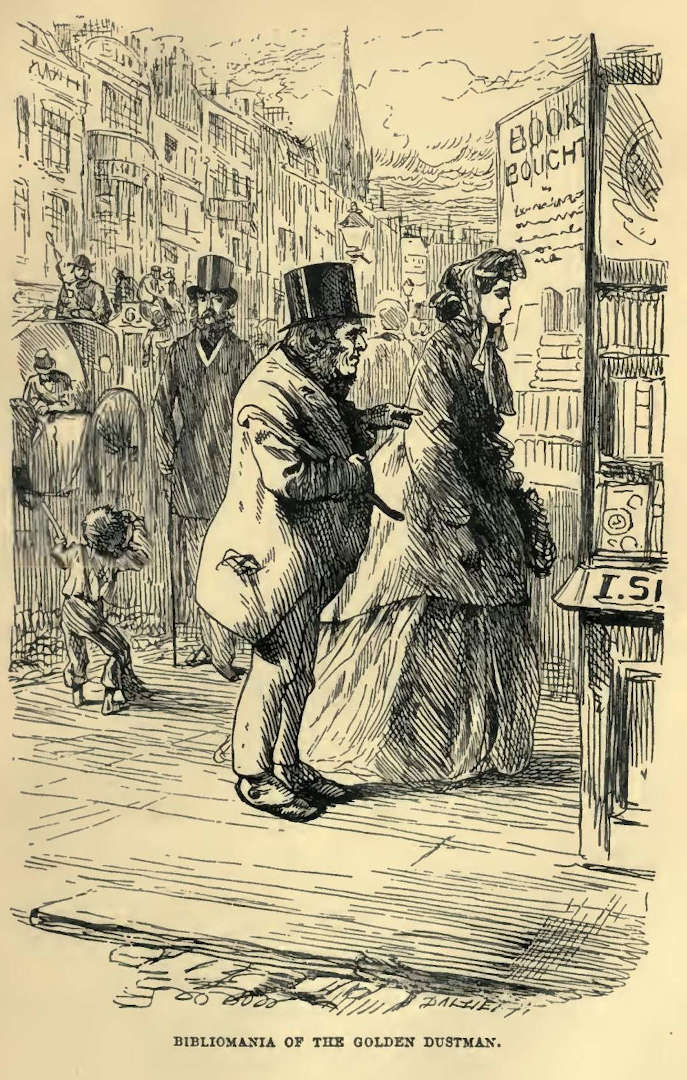
\includegraphics[scale=2.3]{03-05-01}

Chapter 11

IN THE DARK


There was no sleep for Bradley Headstone on that night when Eugene
Wrayburn turned so easily in his bed; there was no sleep for little
Miss Peecher. Bradley consumed the lonely hours, and consumed himself in
haunting the spot where his careless rival lay a dreaming; little Miss
Peecher wore them away in listening for the return home of the master
of her heart, and in sorrowfully presaging that much was amiss with him.
Yet more was amiss with him than Miss Peecher’s simply arranged little
work-box of thoughts, fitted with no gloomy and dark recesses, could
hold. For, the state of the man was murderous.

The state of the man was murderous, and he knew it. More; he irritated
it, with a kind of perverse pleasure akin to that which a sick man
sometimes has in irritating a wound upon his body. Tied up all day with
his disciplined show upon him, subdued to the performance of his routine
of educational tricks, encircled by a gabbling crowd, he broke loose at
night like an ill-tamed wild animal. Under his daily restraint, it was
his compensation, not his trouble, to give a glance towards his state at
night, and to the freedom of its being indulged. If great criminals told
the truth--which, being great criminals, they do not--they would very
rarely tell of their struggles against the crime. Their struggles are
towards it. They buffet with opposing waves, to gain the bloody shore,
not to recede from it. This man perfectly comprehended that he hated his
rival with his strongest and worst forces, and that if he tracked him to
Lizzie Hexam, his so doing would never serve himself with her, or serve
her. All his pains were taken, to the end that he might incense himself
with the sight of the detested figure in her company and favour, in her
place of concealment. And he knew as well what act of his would follow
if he did, as he knew that his mother had borne him. Granted, that he
may not have held it necessary to make express mention to himself of the
one familiar truth any more than of the other.

He knew equally well that he fed his wrath and hatred, and that he
accumulated provocation and self-justification, by being made the
nightly sport of the reckless and insolent Eugene. Knowing all
this,--and still always going on with infinite endurance, pains, and
perseverance, could his dark soul doubt whither he went?

Baffled, exasperated, and weary, he lingered opposite the Temple gate
when it closed on Wrayburn and Lightwood, debating with himself should
he go home for that time or should he watch longer. Possessed in his
jealousy by the fixed idea that Wrayburn was in the secret, if it were
not altogether of his contriving, Bradley was as confident of getting
the better of him at last by sullenly sticking to him, as he would have
been--and often had been--of mastering any piece of study in the way
of his vocation, by the like slow persistent process. A man of rapid
passions and sluggish intelligence, it had served him often and should
serve him again.

The suspicion crossed him as he rested in a doorway with his eyes upon
the Temple gate, that perhaps she was even concealed in that set of
Chambers. It would furnish another reason for Wrayburn’s purposeless
walks, and it might be. He thought of it and thought of it, until
he resolved to steal up the stairs, if the gatekeeper would let him
through, and listen. So, the haggard head suspended in the air flitted
across the road, like the spectre of one of the many heads erst hoisted
upon neighbouring Temple Bar, and stopped before the watchman.

The watchman looked at it, and asked: ‘Who for?’

‘Mr Wrayburn.’

‘It’s very late.’

‘He came back with Mr Lightwood, I know, near upon two hours ago. But if
he has gone to bed, I’ll put a paper in his letter-box. I am expected.’

The watchman said no more, but opened the gate, though rather
doubtfully. Seeing, however, that the visitor went straight and fast in
the right direction, he seemed satisfied.

The haggard head floated up the dark staircase, and softly descended
nearer to the floor outside the outer door of the chambers. The doors
of the rooms within, appeared to be standing open. There were rays of
candlelight from one of them, and there was the sound of a footstep
going about. There were two voices. The words they uttered were not
distinguishable, but they were both the voices of men. In a few moments
the voices were silent, and there was no sound of footstep, and the
inner light went out. If Lightwood could have seen the face which kept
him awake, staring and listening in the darkness outside the door as
he spoke of it, he might have been less disposed to sleep, through the
remainder of the night.

‘Not there,’ said Bradley; ‘but she might have been.’ The head arose to
its former height from the ground, floated down the stair-case again,
and passed on to the gate. A man was standing there, in parley with the
watchman.

‘Oh!’ said the watchman. ‘Here he is!’

Perceiving himself to be the antecedent, Bradley looked from the
watchman to the man.

‘This man is leaving a letter for Mr Lightwood,’ the watchman explained,
showing it in his hand; ‘and I was mentioning that a person had just
gone up to Mr Lightwood’s chambers. It might be the same business
perhaps?’

‘No,’ said Bradley, glancing at the man, who was a stranger to him.

‘No,’ the man assented in a surly way; ‘my letter--it’s wrote by my
daughter, but it’s mine--is about my business, and my business ain’t
nobody else’s business.’

As Bradley passed out at the gate with an undecided foot, he heard it
shut behind him, and heard the footstep of the man coming after him.

‘’Scuse me,’ said the man, who appeared to have been drinking and rather
stumbled at him than touched him, to attract his attention: ‘but might
you be acquainted with the T’other Governor?’

‘With whom?’ asked Bradley.

‘With,’ returned the man, pointing backward over his right shoulder with
his right thumb, ‘the T’other Governor?’

‘I don’t know what you mean.’

‘Why look here,’ hooking his proposition on his left-hand fingers with
the forefinger of his right. ‘There’s two Governors, ain’t there? One
and one, two--Lawyer Lightwood, my first finger, he’s one, ain’t he?
Well; might you be acquainted with my middle finger, the T’other?’

‘I know quite as much of him,’ said Bradley, with a frown and a distant
look before him, ‘as I want to know.’

‘Hooroar!’ cried the man. ‘Hooroar T’other t’other Governor. Hooroar
T’otherest Governor! I am of your way of thinkin’.’

‘Don’t make such a noise at this dead hour of the night. What are you
talking about?’

‘Look here, T’otherest Governor,’ replied the man, becoming hoarsely
confidential. ‘The T’other Governor he’s always joked his jokes agin me,
owing, as I believe, to my being a honest man as gets my living by the
sweat of my brow. Which he ain’t, and he don’t.’

‘What is that to me?’

‘T’otherest Governor,’ returned the man in a tone of injured innocence,
‘if you don’t care to hear no more, don’t hear no more. You begun it.
You said, and likeways showed pretty plain, as you warn’t by no means
friendly to him. But I don’t seek to force my company nor yet my
opinions on no man. I am a honest man, that’s what I am. Put me in the
dock anywhere--I don’t care where--and I says, “My Lord, I am a honest
man.” Put me in the witness-box anywhere--I don’t care where--and I
says the same to his lordship, and I kisses the book. I don’t kiss my
coat-cuff; I kisses the book.’

It was not so much in deference to these strong testimonials to
character, as in his restless casting about for any way or help towards
the discovery on which he was concentrated, that Bradley Headstone
replied: ‘You needn’t take offence. I didn’t mean to stop you. You were
too--loud in the open street; that was all.’

‘’Totherest Governor,’ replied Mr Riderhood, mollified and mysterious,
‘I know wot it is to be loud, and I know wot it is to be soft. Nat’rally
I do. It would be a wonder if I did not, being by the Chris’en name of
Roger, which took it arter my own father, which took it from his own
father, though which of our fam’ly fust took it nat’ral I will not in
any ways mislead you by undertakin’ to say. And wishing that your elth
may be better than your looks, which your inside must be bad indeed if
it’s on the footing of your out.’

Startled by the implication that his face revealed too much of his mind,
Bradley made an effort to clear his brow. It might be worth knowing what
this strange man’s business was with Lightwood, or Wrayburn, or both, at
such an unseasonable hour. He set himself to find out, for the man might
prove to be a messenger between those two.

‘You call at the Temple late,’ he remarked, with a lumbering show of
ease.

‘Wish I may die,’ cried Mr Riderhood, with a hoarse laugh, ‘if I warn’t
a goin’ to say the self-same words to you, T’otherest Governor!’

‘It chanced so with me,’ said Bradley, looking disconcertedly about him.

‘And it chanced so with me,’ said Riderhood. ‘But I don’t mind telling
you how. Why should I mind telling you? I’m a Deputy Lock-keeper up the
river, and I was off duty yes’day, and I shall be on to-morrow.’

‘Yes?’

‘Yes, and I come to London to look arter my private affairs. My private
affairs is to get appinted to the Lock as reg’lar keeper at fust hand,
and to have the law of a busted B’low-Bridge steamer which drownded of
me. I ain’t a goin’ to be drownded and not paid for it!’

Bradley looked at him, as though he were claiming to be a Ghost.

‘The steamer,’ said Mr Riderhood, obstinately, ‘run me down and drownded
of me. Interference on the part of other parties brought me round; but
I never asked ‘em to bring me round, nor yet the steamer never asked ‘em
to it. I mean to be paid for the life as the steamer took.’

‘Was that your business at Mr Lightwood’s chambers in the middle of the
night?’ asked Bradley, eyeing him with distrust.

‘That and to get a writing to be fust-hand Lock Keeper. A recommendation
in writing being looked for, who else ought to give it to me? As I says
in the letter in my daughter’s hand, with my mark put to it to make it
good in law, Who but you, Lawyer Lightwood, ought to hand over this here
stifficate, and who but you ought to go in for damages on my account
agin the Steamer? For (as I says under my mark) I have had trouble
enough along of you and your friend. If you, Lawyer Lightwood, had
backed me good and true, and if the T’other Governor had took me down
correct (I says under my mark), I should have been worth money at the
present time, instead of having a barge-load of bad names chucked at me,
and being forced to eat my words, which is a unsatisfying sort of food
wotever a man’s appetite! And when you mention the middle of the night,
T’otherest Governor,’ growled Mr Riderhood, winding up his monotonous
summary of his wrongs, ‘throw your eye on this here bundle under my arm,
and bear in mind that I’m a walking back to my Lock, and that the Temple
laid upon my line of road.’

Bradley Headstone’s face had changed during this latter recital, and he
had observed the speaker with a more sustained attention.

‘Do you know,’ said he, after a pause, during which they walked on side
by side, ‘that I believe I could tell you your name, if I tried?’

‘Prove your opinion,’ was the answer, accompanied with a stop and a
stare. ‘Try.’

‘Your name is Riderhood.’

‘I’m blest if it ain’t,’ returned that gentleman. ‘But I don’t know
your’n.’

‘That’s quite another thing,’ said Bradley. ‘I never supposed you did.’

As Bradley walked on meditating, the Rogue walked on at his side
muttering. The purport of the muttering was: ‘that Rogue Riderhood, by
George! seemed to be made public property on, now, and that every man
seemed to think himself free to handle his name as if it was a Street
Pump.’ The purport of the meditating was: ‘Here is an instrument. Can I
use it?’

They had walked along the Strand, and into Pall Mall, and had turned
up-hill towards Hyde Park Corner; Bradley Headstone waiting on the pace
and lead of Riderhood, and leaving him to indicate the course. So slow
were the schoolmaster’s thoughts, and so indistinct his purposes when
they were but tributary to the one absorbing purpose or rather when,
like dark trees under a stormy sky, they only lined the long vista at
the end of which he saw those two figures of Wrayburn and Lizzie on
which his eyes were fixed--that at least a good half-mile was traversed
before he spoke again. Even then, it was only to ask:

‘Where is your Lock?’

‘Twenty mile and odd--call it five-and-twenty mile and odd, if you
like--up stream,’ was the sullen reply.

‘How is it called?’

‘Plashwater Weir Mill Lock.’

‘Suppose I was to offer you five shillings; what then?’

‘Why, then, I’d take it,’ said Mr Riderhood.

The schoolmaster put his hand in his pocket, and produced two
half-crowns, and placed them in Mr Riderhood’s palm: who stopped at
a convenient doorstep to ring them both, before acknowledging their
receipt.

‘There’s one thing about you, T’otherest Governor,’ said Riderhood,
faring on again, ‘as looks well and goes fur. You’re a ready money man.
Now;’ when he had carefully pocketed the coins on that side of himself
which was furthest from his new friend; ‘what’s this for?’

‘For you.’

‘Why, o’ course I know THAT,’ said Riderhood, as arguing something that
was self-evident. ‘O’ course I know very well as no man in his right
senses would suppose as anythink would make me give it up agin when I’d
once got it. But what do you want for it?’

‘I don’t know that I want anything for it. Or if I do want anything
for it, I don’t know what it is.’ Bradley gave this answer in a stolid,
vacant, and self-communing manner, which Mr Riderhood found very
extraordinary.

‘You have no goodwill towards this Wrayburn,’ said Bradley, coming to
the name in a reluctant and forced way, as if he were dragged to it.

‘No.’

‘Neither have I.’

Riderhood nodded, and asked: ‘Is it for that?’

‘It’s as much for that as anything else. It’s something to be agreed
with, on a subject that occupies so much of one’s thoughts.’

‘It don’t agree with YOU,’ returned Mr Riderhood, bluntly. ‘No! It
don’t, T’otherest Governor, and it’s no use a lookin’ as if you wanted
to make out that it did. I tell you it rankles in you. It rankles in
you, rusts in you, and pisons you.’

‘Say that it does so,’ returned Bradley with quivering lips; ‘is there
no cause for it?’

‘Cause enough, I’ll bet a pound!’ cried Mr Riderhood.

‘Haven’t you yourself declared that the fellow has heaped provocations,
insults, and affronts on you, or something to that effect? He has done
the same by me. He is made of venomous insults and affronts, from the
crown of his head to the sole of his foot. Are you so hopeful or so
stupid, as not to know that he and the other will treat your application
with contempt, and light their cigars with it?’

‘I shouldn’t wonder if they did, by George!’ said Riderhood, turning
angry.

‘If they did! They will. Let me ask you a question. I know something
more than your name about you; I knew something about Gaffer Hexam. When
did you last set eyes upon his daughter?’

‘When did I last set eyes upon his daughter, T’otherest Governor?’
repeated Mr Riderhood, growing intentionally slower of comprehension as
the other quickened in his speech.

‘Yes. Not to speak to her. To see her--anywhere?’

The Rogue had got the clue he wanted, though he held it with a clumsy
hand. Looking perplexedly at the passionate face, as if he were trying
to work out a sum in his mind, he slowly answered:

‘I ain’t set eyes upon her--never once--not since the day of Gaffer’s
death.’

‘You know her well, by sight?’

‘I should think I did! No one better.’

‘And you know him as well?’

‘Who’s him?’ asked Riderhood, taking off his hat and rubbing his
forehead, as he directed a dull look at his questioner.

‘Curse the name! Is it so agreeable to you that you want to hear it
again?’

‘Oh! HIM!’ said Riderhood, who had craftily worked the schoolmaster into
this corner, that he might again take note of his face under its evil
possession. ‘I’d know HIM among a thousand.’

‘Did you--’ Bradley tried to ask it quietly; but, do what he might
with his voice, he could not subdue his face;--‘did you ever see them
together?’

(The Rogue had got the clue in both hands now.)

‘I see ‘em together, T’otherest Governor, on the very day when Gaffer
was towed ashore.’

Bradley could have hidden a reserved piece of information from the sharp
eyes of a whole inquisitive class, but he could not veil from the eyes
of the ignorant Riderhood the withheld question next in his breast.
‘You shall put it plain if you want it answered,’ thought the Rogue,
doggedly; ‘I ain’t a-going a wolunteering.’

‘Well! was he insolent to her too?’ asked Bradley after a struggle. ‘Or
did he make a show of being kind to her?’

‘He made a show of being most uncommon kind to her,’ said Riderhood. ‘By
George! now I--’

His flying off at a tangent was indisputably natural. Bradley looked at
him for the reason.

‘Now I think of it,’ said Mr Riderhood, evasively, for he was
substituting those words for ‘Now I see you so jealous,’ which was the
phrase really in his mind; ‘P’r’aps he went and took me down wrong, a
purpose, on account o’ being sweet upon her!’

The baseness of confirming him in this suspicion or pretence of one (for
he could not have really entertained it), was a line’s breadth beyond
the mark the schoolmaster had reached. The baseness of communing and
intriguing with the fellow who would have set that stain upon her, and
upon her brother too, was attained. The line’s breadth further, lay
beyond. He made no reply, but walked on with a lowering face.

What he might gain by this acquaintance, he could not work out in his
slow and cumbrous thoughts. The man had an injury against the object of
his hatred, and that was something; though it was less than he supposed,
for there dwelt in the man no such deadly rage and resentment as burned
in his own breast. The man knew her, and might by a fortunate chance see
her, or hear of her; that was something, as enlisting one pair of eyes
and ears the more. The man was a bad man, and willing enough to be in
his pay. That was something, for his own state and purpose were as
bad as bad could be, and he seemed to derive a vague support from the
possession of a congenial instrument, though it might never be used.

Suddenly he stood still, and asked Riderhood point-blank if he knew
where she was? Clearly, he did not know. He asked Riderhood if he would
be willing, in case any intelligence of her, or of Wrayburn as seeking
her or associating with her, should fall in his way, to communicate it
if it were paid for? He would be very willing indeed. He was ‘agin ‘em
both,’ he said with an oath, and for why? ‘Cause they had both stood
betwixt him and his getting his living by the sweat of his brow.

‘It will not be long then,’ said Bradley Headstone, after some more
discourse to this effect, ‘before we see one another again. Here is the
country road, and here is the day. Both have come upon me by surprise.’

‘But, T’otherest Governor,’ urged Mr Riderhood, ‘I don’t know where to
find you.’

‘It is of no consequence. I know where to find you, and I’ll come to
your Lock.’

‘But, T’otherest Governor,’ urged Mr Riderhood again, ‘no luck never
come yet of a dry acquaintance. Let’s wet it, in a mouth-fill of rum and
milk, T’otherest Governor.’

Bradley assenting, went with him into an early public-house, haunted by
unsavoury smells of musty hay and stale straw, where returning carts,
farmers’ men, gaunt dogs, fowls of a beery breed, and certain human
nightbirds fluttering home to roost, were solacing themselves after
their several manners; and where not one of the nightbirds hovering
about the sloppy bar failed to discern at a glance in the passion-wasted
nightbird with respectable feathers, the worst nightbird of all.

An inspiration of affection for a half-drunken carter going his way led
to Mr Riderhood’s being elevated on a high heap of baskets on a waggon,
and pursuing his journey recumbent on his back with his head on his
bundle. Bradley then turned to retrace his steps, and by-and-by struck
off through little-traversed ways, and by-and-by reached school and
home. Up came the sun to find him washed and brushed, methodically
dressed in decent black coat and waistcoat, decent formal black tie, and
pepper-and-salt pantaloons, with his decent silver watch in its pocket,
and its decent hair-guard round his neck: a scholastic huntsman clad for
the field, with his fresh pack yelping and barking around him.

Yet more really bewitched than the miserable creatures of the
much-lamented times, who accused themselves of impossibilities under a
contagion of horror and the strongly suggestive influences of Torture,
he had been ridden hard by Evil Spirits in the night that was newly
gone. He had been spurred and whipped and heavily sweated. If a record
of the sport had usurped the places of the peaceful texts from Scripture
on the wall, the most advanced of the scholars might have taken fright
and run away from the master.



